

\section{Theorie}
\label{sec:Theorie}

Der Frequenzbereich des Ultraschalls reicht von ca. 20 \si{\kilo\hertz} bis ca. 1 \si{\giga\hertz}.
Schall bewegt sich durch Druckschwankungen fort und ist eine longitudinale Welle
\begin{equation}
p(x,t) = p_0 + v_0 Z cos(\omega t - kx) ,
\end{equation}
wobei $Z = c \cdot \rho $ die akustische Impedanz ist, mit \rho als Dichte des Materials.
Die Schallgeschwindigkeit wird durch die Variable $c$ beschrieben.
Diese hängt in Flüssigkeiten von der Kompressibilität \kappa und der Dichte \rho der Flüssigkeit ab:
\begin{equation}
c_{F_l} = \sqrt{\frac{1}{\kappa \cdot \rho}} ,
\end{equation}
und in einem Festkörper von dem Elastizitätsmodul $E$
\begin{equation}
c_{F_k} = \sqrt{\frac{E}{\rho}} .
\end{equation}
Auf Grund von Schubspannungen breiten sich die Schallwellen in Festkörpern auch als Transversalwellen aus.
Da sich Schall wie eine elektromagnetische Welle verhält, können Reflexion und Brechnung auftreten.
Der Reflexionskoeffizient $R$ bestimmt sich aus der Impedanz der beiden Materialien
\begin{equation}
R = (\frac{Z_1 - Z_2}{Z_1 + Z_2})^2 .
\end{equation}
Aus der Relation
\begin{equation}
T + R = 1 ,
\end{equation}
lässt sich der Transmittierte Teil $T$ berechnen.
Ein Teil ihrer Energie geht durch Absorption verloren, und somit nimmt die Intensität exponentiell nach der Strecke $x$ ab:
\begin{equation}
I(x) = I_0 \cdot e^{\alpha x} ,
\end{equation}
wobei \alpha der Absorptionskoeffizient der Schallamplitude ist. Auf Grund dieser Absorption vor allem in Luft, wird ein Kontaktmittel zwischen Schallgeber und untersuchendem Material verwendet.

Ultraschall kann zum Beispiel durch den piezo-elektrischen Effekt erzeugt werden. 
Dazu wird ein Piezokristall ineinem elektrischen Wechselfeld zu Schwingungen angeregt, wobei Ultraschallwellen abgestrahlt werden.

In der Ultraschalltechnik werden zwei Verfahren angewendet, welche in Abbildung (1) schematisch dargestellt sind.
Bei dem Durchschallungs-Verfahren werden der Schallimpuls und der Empfangsimpuls aufgefangen. Ob sich eine Fehlstelle in der Probe befindet, erkennt man an der Messung einer schwächeren Intensität am Empfänger.
Anders als beim Durchschallungs-Verfahren, kann beim Impuls-Echo-Verfahren die Lage und Größe der Fehlstelle bestimmt werden. Der Sender ist hier gleichzeitig auch der Empfänger. Der Impuls wird reflektiert und vom Empfänger wieder aufgenommen.
Je nachdem wie hoch das Echo ist, kann man die Größe der Fehlstelle bestimmen.
Die Lage der Fehlstelle wird über
\begin{equation}
s = \frac{1}{2}ct .
\end{equation}

Drei verschiedene Darstellungsarten können die Laufzeit darstellen.
Mit dem A-Scan (Amplituden Scan) werden die Amplituden des Echos in Abhängigkeit der Laufzeit dargestellt.
Der B-Scan (Brightness Scan) stellt die Amplituden in Helligkeitsabstufungen dar, wobei ein zweidimensionales Bild entsteht.
Mit dem TM-Scan (Time-Motion Scan) kann eine zeitliche Bildfolge aufgenommen werden.

\begin{figure}[H]
  \centering
  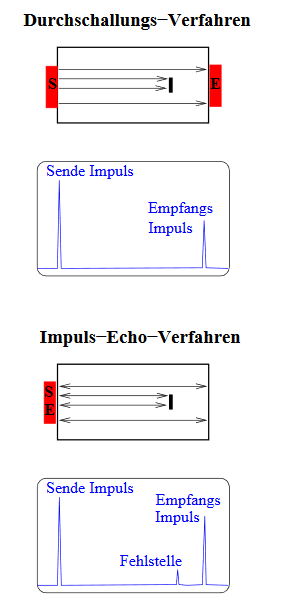
\includegraphics[height=8cm]{verfahren.png}
  \caption{Schema des Durchschallungs- und des Impuls-Echo-Verfahrens. \cite[S.2]{kent}}
\end{figure}


